\documentclass[12pt,a4paper,utf8x]{report}
\usepackage [frenchb]{babel}

% Pour pouvoir utiliser 
\usepackage{ucs}
\usepackage[utf8x]{inputenc}
\usepackage{graphicx}

\usepackage{url} % Pour avoir de belles url
\usepackage {geometry}

% Pour mettre du code source
\usepackage {listings}
% Pour pouvoir passer en paysage
\usepackage{lscape}

% Pour pouvoir faire plusieurs colonnes
\usepackage {multicol}
% Pour crééer un index
\usepackage{makeidx}
\makeindex

% Pour gérer les liens interractifs et les signets Acrobat
\usepackage{hyperref}
\hypersetup{
pdftitle={Rapport projet ALMA-TWE},
pdfauthor={Nom de l'auteur},
pdfsubject={Sujet du document},
pdfkeywords={les mots clefs},
bookmarks, % Création du signet
pdfstartview=FitH, % Page de la largeur de la fenêtre
colorlinks=true, % Liens en couleur
linkcolor=black, 	
anchorcolor=black, 	
citecolor=black, 	
filecolor=black, 	
menucolor=black,
runcolor=black,
urlcolor=black, 	
frenchlinks=black,
bookmarksnumbered=true, % Signet numéroté
pdfpagemode=UseOutlines, % Montre les bookmarks.
bookmarksopen =true,
}

% Pour afficher la bibliographie, mais pas nottoc (Table of Contents), notlof (List of Figures) ni notlot (List of Tables)
\usepackage[notlof, notlot]{tocbibind}


% Pour les entetes de page
% \usepackage{fancyheadings}
%\pagestyle{fancy}
%\renewcommand{\sectionmark}[1]{\markboth{#1}{}} 
%\renewcommand{\subsectionmark}[1]{\markright{#1}} 

% Pour l'interligne de 1.5
\usepackage {setspace}
% Pour les marges de la page
\geometry{a4paper, top=2.5cm, bottom=3.5cm, left=1.5cm, right=1.5cm, marginparwidth=1.2cm}

\parskip=5pt %% distance entre § (paragraphe)
\sloppy %% respecter toujours la marge de droite 

% Pour les pénalités :
\interfootnotelinepenalty=150 %note de bas de page
\widowpenalty=150 %% veuves et orphelines
\clubpenalty=150 

%Pour la longueur de l'indentation des paragraphes
\setlength{\parindent}{15mm}



%%%% debut macro pour enlever le nom chapitre %%%%
\makeatletter
\def\@makechapterhead#1{%
  \vspace*{50\p@}%
  {\parindent \z@ \raggedright \normalfont
    \interlinepenalty\@M
    \ifnum \c@secnumdepth >\m@ne
        \Huge\bfseries \thechapter\quad
    \fi
    \Huge \bfseries #1\par\nobreak
    \vskip 40\p@
  }}

\def\@makeschapterhead#1{%
  \vspace*{50\p@}%
  {\parindent \z@ \raggedright
    \normalfont
    \interlinepenalty\@M
    \Huge \bfseries  #1\par\nobreak
    \vskip 40\p@
  }}
\makeatother
%%%% fin macro %%%%

%Couverture 

\title
{
	\normalsize{Rapport de projet\\
	Service\\
	Université de Nantes\\
	2010-2011}\\
	\vspace{15mm}
	\Huge{ALMA-TWE}
}
\author{DEJEAN Charles, POTTIER Vincent\\
	\vspace{45mm}
}


\begin{document}

\maketitle
%Remerciements

Je tiens à remercier :
et on met la liste des personnes que l'on remercie. Toto, tutu, titi. et on met la liste des personnes que l'on remercie. Toto, tutu, titi.et on met la liste des personnes que l'on remercie. Toto, tutu, titi.et on met la liste des personnes que l'on remercie. Toto, tutu, titi.


Et on met la liste des personnes que l'on remercie. Toto, tutu, titi.et on met la liste des personnes que l'on remercie. Toto, tutu, titi.et on met la liste des personnes que l'on remercie. Toto, tutu, titi.et on met la liste des personnes que l'on remercie. Toto, tutu, titi.et on met la liste des personnes que l'on remercie. Toto, tutu, titi.

%\clearpage

\tableofcontents
\clearpage

% Pour avoir un interligne de 1,5
\begin{onehalfspace}

\chapter{Architecture}

	Le projet ALMA-TWE est composé de plusieurs parties indépendantes les une des
	autres. Commençons donc par voir l'architecture générale de l'application et
	comment ses différentes parties intéragissent entre elles.

	\section{Vue générale}
	
		\begin{figure}[!h]
			\centering
			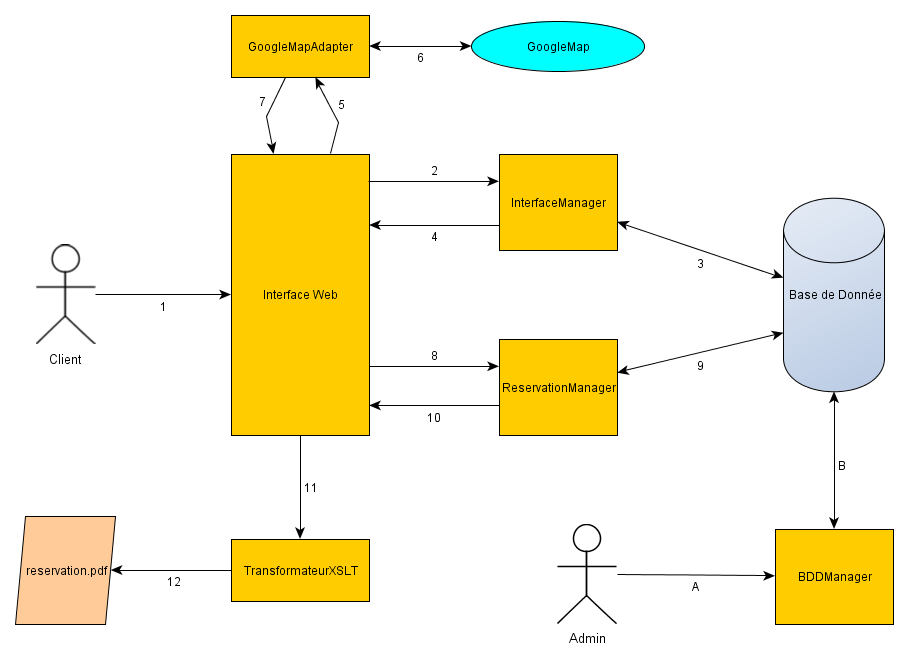
\includegraphics[width=1\textwidth]{overview}
			\label{overview}
		\end{figure}
		
	\section{Base de donnée}
		
		\begin{figure}[!h]
			\centering
			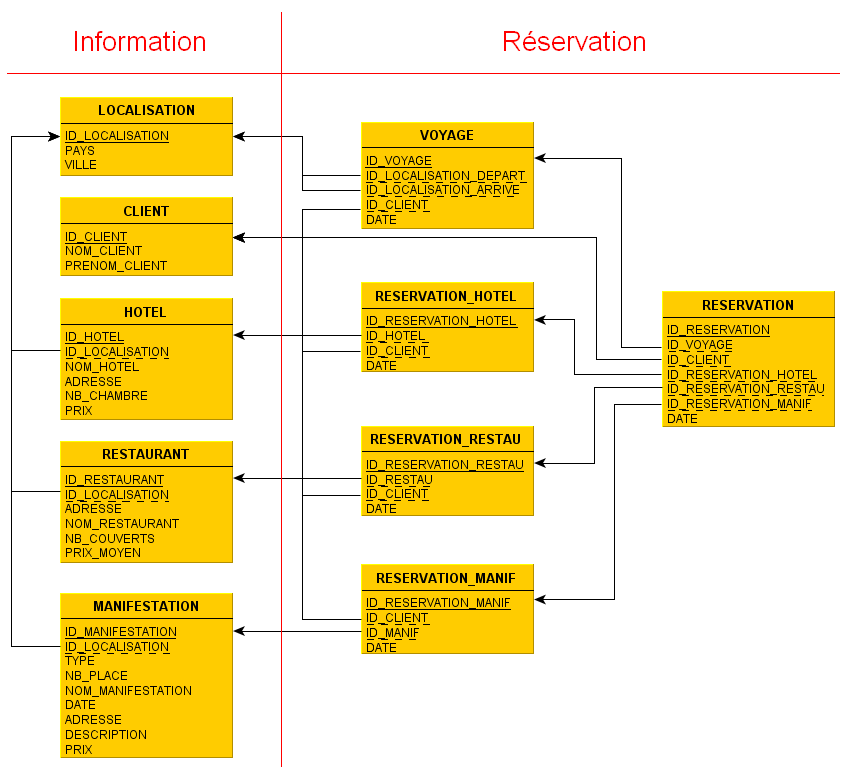
\includegraphics[width=1\textwidth]{bdd}
		\end{figure}
		
		Notre base de donnée contient deux types de tables :
		
		\begin{itemize}
		  \item Information, contenant les informations fixes de notre système. Elles
		  ne seront modifiables que par l'administrateur. 
		  \item Réservation, contenant les réservations faites par les clients.
		\end{itemize}
			
	\section{InterfaceWeb}
		
		L'interface consiste en un formulaire que le client va remplir
		(figure \ref{overview}, flèche 1 ) . A chaque modification du formulaire
		, il va se mettre à jour grâce au service InterfaceManager (figure
		\ref{overview}, flèches 2 et 4)
		
		Une fois toute les informations remplies, il est possible de visualiser les
		différentes adresses sur une carte, via un service GoogleMap (figure
		\ref{overview}, flèches 5 et 6)
		
		A la fin, le Client pourra valider sa réservation. Cela activera le service
		ReservationManager (figure \ref{overview}, flèches 7 et 9). Il enregistrera
		pour finir la réservation dans la Base de donnée, si possible, et retournera
		le résultat.
		
		Pour finir si la réservation est un succès, un résumé de celle-ci sera
		sauvegardé au format pdf (figure \ref{overview}, flèche 10).
	
	\section{InterfaceManager}
	
		\subsection{Fonctionnement}
	
			L'interfaceManager est un service qui récupère en entrée (figure
			\ref{overview}, flèche 2) toujours le méme format de donnée, et qui en
			fonction des champs plein ou vide recherchera dans la base de donnée
			(figure\ref{overview}, flèche 3) les information complémentaire, et les
			retournera à l'Interface (figure\ref{overview}, flèche 4).
		
		\subsection{Format des données}
		
			En entrée (figure\ref{overview}, flèche 2):
			\begin{itemize}
			  \item Pays
			  \item Ville
			  \item Date
			  \item Type de Manifestation\\
			\end{itemize}
			
			En sortie (figure\ref{overview}, flèche 4):
			\begin{itemize}
			  \item Pays
			  \item Villes
			  \item Type de Manifestations
			  \item Manifestations (Id,Nom,Adresse,Description,Prix,Places)
			  \item Hotels (Id,Nom,Adresse,Nombre de chambres,Prix)
			  \item Restaurants (Id,Nom,Adresse,Nombre de couvert,Prix moyen)
			\end{itemize}
		
		\subsection{Dépendances}
		
			Si le champs Pays de la requète est vide, InterfaceManager
			renvera la liste des pays contenues dans la base de donnée.
			
			Si le champs Pays est complété et que le champs Ville est vide,
			InterfaceManager renvera la liste des villes du pays spécifiée contenues dans
			la base de donnée.
		
			Si les champs Pays, Ville et Date sont complété et que le champs Type de
			Manifestations est vide, InterfaceManager renvera la liste des Type de
			Manifestations qui auront lieu dans cette Ville a cette Date.
			
			Enfin si tout les champs sont remplis InterfaceManager renvera la liste des
			Manifestation qui auront lieu dans cette Ville a cette Date et des Hotels et
			Restaurants de cette ville.
		
	\section{ReservationManager}	
	
		\subsection{Fonctionnement}
	
			Ce service sert à enregistrer, dans la base de données, les réservations
			choisis par le client. On lui envoie les Id de chaque élément à
			reserver(figure\ref{overview}, flèche 7), il vérifie que les reservations
			sont possible et si tout est OK il les éffectue(figure\ref{overview}, flèche
			8). Enfin il retourne un message confimant ou non la
			reservation(figure\ref{overview}, flèche 9).
	
		\subsection{Format des données}
		
			En entrée (figure\ref{overview}, flèche 7):
			\begin{itemize}
			  \item Nom
			  \item Prenom
			  \item IdManif
			  \item IdHotel
			  \item IdRestau
			  \item Voyage(Pays de Départ, Ville de Départ, Pays d'Arrivée, Ville de
			  d'Arrivée)\\
			\end{itemize}
	
			En sortie une simple chaine de caractère.
	
	\section{BDDManager}
		
		
\clearpage

\chapter{Implémentation}

\section{Interface Web}

Nous avons utilisé la technologie JSF pour faire l'Interface Web. cela a été
grandement simplifié par l'utilisation du Plugin Visual JSF, qui permet de créer
une interface graphique et le code associé très facilement.

Pour l'image Google Map, elle a été créée à partir du service Static Maps API
V2.\\

\begin{figure}[!h]
	\centering
	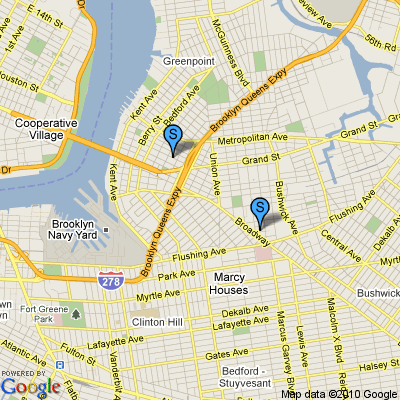
\includegraphics[scale=0.5]{staticmap.png}
	\caption{exemple d'image Google Map}
	\label{staticmap}
\end{figure}

Le principe est simple : il suffit de construire une url selon une méthodologie
particulière, et de la déclarer en tant qu'image url. Il est possible de
construire ainsi des url plutôt complexe permettant d'afficher des chemins
prédéfinis, les routes, \ldots

\clearpage

Par exemple, l'url permettant d'afficher l'exemple de l'image précédente :

\begin{verbatim}
http://maps.google.com/maps/api/staticmap?
center=Brooklyn+Bridge,New+York,NY
&zoom=14&size=512x512
&maptype=roadmap
&markers=color:blue|label:S|40.702147,-74.015794
&markers=color:green|label:G|40.711614,-74.012318
&markers=color:red|color:red|label:C|40.718217,-73.998284
&sensor=false
\end{verbatim}



\section{Web Services}

	\subsection{InterfaceManager}
	
		Ce service est un BPEL simple, qui effectue des requetes FIND dans les tables
		de type Information (figure\ref{bdd}) en fonction des champ remplie dans la
		requete.
	
	\subsection{ReservationManager}

		Ce service est une application composite de BPEL, qui comprend :
		\begin{itemize}
		  \item ReservationManager : BPEL central, il permet de coordonné tout les
		  autres BPEL et qui enregistre la reservation des reservations.
		  \item ClientManager : BPEL qui vérifie l'existance d'un client et qui
		  permet de récupérer son Id en partant de ses nom et prenom.
		  \item ReservManif : BPEL qui vérifie qu'une manifestation existe et qu'il y
		  a encors de la place. Et enregistre une reservation pour cette
		  manifestation.
		  \item ReservHotel : BPEL qui vérifie qu'un hotel existe et qu'il y a encors
		  de la place à une date donnée. Et enregistre une reservation pour cet
		  hotel.
		  \item ReservRestau : BPEL qui vérifie qu'un restaurant existe et qu'il y a
		  encors de la place à une date donnée. Et enregistre une reservation pour ce
		  restaurant.
		\end{itemize}
		
		les vérifications sont effectué grâce à toutes les tables, et les reservation
		sont enregistrées dans les tables de type Réservation (figure\ref{bdd}).
		
		Si une reservation est un succès ReservationManager renvoie 'OK' a l'Interface
		sinon un message d'erreur précisant le problème.

\section{BDD Manager}

\clearpage






















% Pour finir l'interligne de 1,5
\end{onehalfspace}

%----------------------------------------
% Pour la bibliographie
%----------------------------------------
% Citer tous les ouvrages/références
% \nocite{*}
% Trier par ordre d'apparition
% \bibliographystyle{unsrt}
% Pour le style de la biblio
% \bibliographystyle{plain.bst}
% Ecrire la biblio ici
% \bibliography{biblio}

\printindex

\appendix


\end{document}
